\chapter{Нарушенная симметрия, бозоны Голдстоуна и калибровочная инвариантность}

Мы хотим понять, как частица, подобная фотону, может приобрести массу. Именно к этому мы хотим прийти, но начинать с этого неразумно. Прямой массовый член для калибровочного поля, по-видимому, разрушает ту самую калибровочную инвариантность, которая делает теорию состоятельной. Прежде чем мы увидим путь выхода, нам нужны две идеи в рабочем виде:
\begin{enumerate}
  \item спонтанное нарушение симметрии, особенно для непрерывной симметрии;
  \item калибровочная инвариантность, при которой операция симметрии может меняться от одной точки пространства-времени к другой.
\end{enumerate}
Ни одну из этих идей нельзя заменить лозунгом. Первую мы построим на примере магнита, переведём её на язык теории скалярного поля и обнаружим безмассовую моду Голдстоуна. Затем мы возьмём ту же симметрию \(U(1)\) и сделаем её локальной, что вынудит нас ввести векторный потенциал и ковариантную производную. Лишь в конце мы поставим рядом обе линии рассуждения. Их действительное объединение---явление Хиггса---составляет предмет следующей лекции.

\section{Симметричный закон с асимметричным основным состоянием}

\subsection{Магнит с двумя состояниями}

Начнём с решётки маленьких магнитов. Каждый спин может быть ориентирован вверх или вниз, и соседние спины понижают свою энергию, если направлены в одну и ту же сторону. В трёхмерной кубической решётке у спина шесть ближайших соседей, но точное координационное число несущественно. Существенно правило
\begin{equation}
  E_{\parallel}<E_{\rm antiparallel}.
\end{equation}
Микроскопическое правило не меняется, если обратить каждый спин:
\begin{equation}
  \uparrow\longleftrightarrow\downarrow.
\end{equation}
Тем не менее конфигурации с наименьшей энергией сами по себе несимметричны. Это
\begin{equation}
  \{\uparrow\uparrow\uparrow\cdots\},
  \qquad
  \{\downarrow\downarrow\downarrow\cdots\}.
\end{equation}
Уравнения допускают обе, но холодный макроскопический образец должен выбрать одну.

Этот выбор чрезвычайно чувствителен. Зафиксируйте один спин очень далеко так, чтобы он указывал вверх. Его соседи предпочитают следовать за ним, их соседи предпочитают следовать за ними, и эта информация распространяется по всему образцу. Возмущение, сколь угодно малое по сравнению со всей системой, может выбрать ориентацию всего основного состояния. Именно эта неустойчивость и имеется в виду под \emph{спонтанным} нарушением симметрии.

\begin{classroomqa}
\audiencequestion{Может ли нейтральная частица ориентироваться в магнитном поле?
\lecturetimestamp{00:05:14}}
\lecturerresponse{Да. Электрическая нейтральность не означает отсутствия магнитного момента. Нейтрон нейтрален, но обладает магнитным моментом из-за своих внутренних заряженных составляющих. Поэтому магнитное поле может различать ориентации его спина.}
\end{classroomqa}

\begin{classroomqa}
\audiencequestion{Если система меняет ориентацию, происходит ли это изменение сразу повсюду? Могут ли сосуществовать несколько волн переориентации?
\lecturetimestamp{00:05:41--00:06:38}}
\lecturerresponse{Изменение распространяется. Одна область увлекает своих соседей, почти как трёхмерный массив костяшек домино, и возмущение распространяется в виде волны. Разные области могут начать выбор независимо, так что до того, как победит одна ориентация, могут существовать несколько фронтов и несколько доменов. К этим самым волнам мы вернёмся, когда симметрия станет непрерывной.}
\end{classroomqa}

\subsection{Явное нарушение — это другая теория}

Теперь поместим образец во внешнее магнитное поле, направленное вверх. У изолированного спина энергия уже меньше, когда он направлен вверх. Преобразование \(\uparrow\leftrightarrow\downarrow\) больше не оставляет энергию неизменной: предпочтение встроено в сам закон. Это \emph{явное} нарушение симметрии.

Различие можно проверить, не зная, как был приготовлен образец. Возьмите очень большой образец, удерживайте его левую границу в состоянии «вверх», а правую — в состоянии «вниз». Если магнитное поле во всём объёме явно предпочитает «вверх», правое граничное условие проникает лишь на малое расстояние. Макроскопическая область «вниз» потребовала бы энергии, пропорциональной её объёму, так что объём образца не может оставаться разделённым на две одинаково выгодные фазы.

Без внешнего смещения «вверх» и «вниз» имеют одну и ту же объёмную энергию. Тогда состояние с наименьшей энергией при таких ограничениях содержит домен «вверх», домен «вниз» и конечный переходный слой между ними. Интерфейс не обязан находиться в геометрическом центре, но нет объёмного давления, заставляющего одну фазу уничтожить другую. Этот интерфейс — \emph{доменная стенка}, характерный дефект этой нарушенной дискретной симметрии.

\begin{figure}[htbp]
\centering
\begin{adjustbox}{max width=\linewidth}
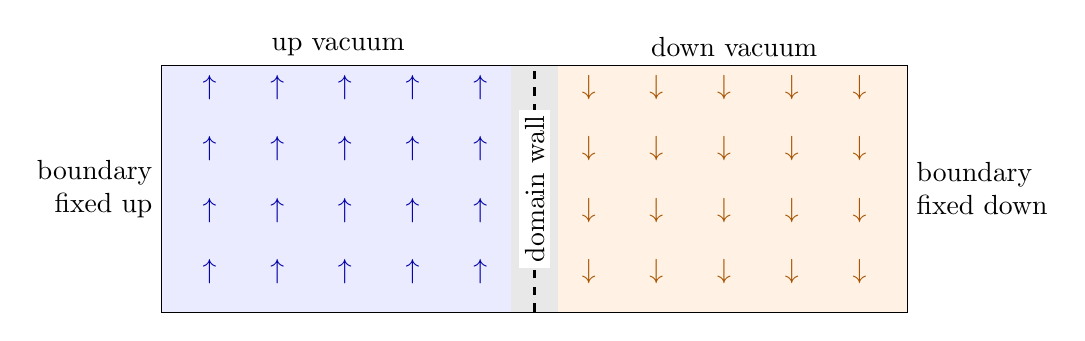
\begin{tikzpicture}[x=0.86cm,y=0.78cm]
  \draw[thick] (0,0) rectangle (11,4);
  \fill[blue!8] (0,0) rectangle (5.15,4);
  \fill[orange!10] (5.85,0) rectangle (11,4);
  \fill[gray!18] (5.15,0) rectangle (5.85,4);
  \foreach \x in {0.7,1.7,2.7,3.7,4.7}
    \foreach \y in {0.65,1.65,2.65,3.65}
      \node[blue!65!black] at (\x,\y) {$\uparrow$};
  \foreach \x in {6.3,7.3,8.3,9.3,10.3}
    \foreach \y in {0.65,1.65,2.65,3.65}
      \node[orange!65!black] at (\x,\y) {$\downarrow$};
  \draw[dashed,thick] (5.5,0) -- (5.5,4);
  \node[above] at (2.6,4) {up vacuum};
  \node[above] at (8.45,4) {down vacuum};
  \node[rotate=90,fill=white,inner sep=2pt] at (5.5,2) {domain wall};
  \node[left,align=right] at (0,2) {boundary\\fixed up};
  \node[right,align=left] at (11,2) {boundary\\fixed down};
\end{tikzpicture}
\end{adjustbox}
\caption{Граничный тест на спонтанное нарушение дискретной симметрии. Обе ориентации в объёме имеют одинаковую энергию, поэтому стенка может разделять макроскопические домены.}
\end{figure}

\begin{classroomqa}
\audiencequestion{Требует ли этот аргумент взаимодействий только между ближайшими соседями?\lecturetimestamp{00:18:18}}
\lecturerresponse{Нет. Взаимодействие со вторыми соседями, которое тоже благоприятствует выравниванию, меняет детали, но не вывод. Более интересное поведение возникает, если взаимодействия на разных расстояниях конкурируют---например, ближайшие соседи предпочитают выравнивание, а следующие за ближайшими — противоположную ориентацию. Это приводит к фрустрации и более сложным упорядоченным фазам, но не меняет основного различия, о котором здесь идёт речь.}
\end{classroomqa}

\begin{classroomqa}
\audiencequestion{Относится ли \emph{спонтанное} к большой производной внутри стенки?\lecturetimestamp{00:19:05}}
\lecturerresponse{Нет. Оно относится к тому, что сама энергия не имеет предпочтения вверх--вниз, тогда как у выбранного основного состояния оно есть. Резкий отклик на сколь угодно малое возмущение выявляет неустойчивость. Градиент лишь говорит нам, во что обходится интерфейс.}
\end{classroomqa}

\begin{classroomqa}
\audiencequestion{Находился ли материал уже в одном из двух состояний, или его состояние изначально было неизвестно?\lecturetimestamp{00:19:40}}
\lecturerresponse{Это зависит от его истории. При высокой температуре тепловое движение может оставить спины «вверх» и «вниз» перемешанными, так что средняя намагниченность почти равна нулю. По мере охлаждения материала разные области выбирают разные ориентации, образуются доменные стенки, и домены укрупняются. Случайность и крошечные возмущения окружающей среды определяют, какой вакуум в конце концов займёт большую часть образца.}
\end{classroomqa}

\section{Тот же аргумент в теории скалярного поля}

Заменим спины вещественным скалярным полем \(\phi(\bm{x},t)\). Зафиксировав раз и навсегда соглашения о метрике и нормировке, запишем
\begin{equation}
\begin{aligned}
  \mathcal L
  &=\frac12\,\partial_\mu\phi\,\partial^\mu\phi-V(\phi),
  \\
  \mathcal E
  &=\frac12\dot\phi^{\,2}+\frac12(\nabla\phi)^2+V(\phi).
\end{aligned}
  \label{eq:l07-real-scalar}
\end{equation}
Релятивистская сокращённая запись в \(\mathcal L\) содержит положительный член с производной по времени и отрицательный член с пространственным градиентом; в гамильтоновой плотности энергии оба вклада положительны.

Выберем чётный потенциал с двумя вырожденными минимумами,
\begin{equation}
  V(\phi)=\frac{\lambda}{4}\left(\phi^2-f^2\right)^2,
  \qquad \lambda>0.
  \label{eq:l07-double-well}
\end{equation}
Лагранжиан инвариантен относительно \(\phi\mapsto-\phi\), тогда как любой из двух однородных вакуумов
\begin{equation}
  \phi(\bm{x})=+f,
  \qquad\hbox{or}\qquad
  \phi(\bm{x})=-f
\end{equation}
выбирает одну из двух сторон. Потенциал с единственным минимумом при \(\phi=0\), напротив, имеет симметричный вакуум, и спонтанного нарушения в этом случае нет.

Зафиксируем \(\phi=+f\) на одной стороне образца и \(\phi=-f\) на другой. Поле не может совершить скачок без энергетической цены, поскольку
\begin{equation}
  E_{\rm wall}
  =\int dx\left[
      \frac12\left(\frac{d\phi}{dx}\right)^2+V(\phi)-V(f)
    \right].
  \label{eq:l07-wall-energy}
\end{equation}
Резкий скачок делает \(d\phi/dx\) чрезвычайно большим. Поэтому стенка минимальной энергии распределяет изменение по конечной ширине, уравновешивая градиентную энергию и потенциальную цену прохождения между минимумами. Хорошо известное кинк-решение для потенциала в уравнении ~\eqref{eq:l07-double-well} имеет вид
\begin{equation}
  \phi_{\rm wall}(x)
  =f\tanh\!\left[f\sqrt{\frac{\lambda}{2}}\,(x-x_0)\right],
  \label{eq:l07-kink}
\end{equation}
и даёт явную реализацию плавного перехода, описанного у доски.
\editorialnote{В лекции рассуждение строится по форме потенциала и градиентному члену, но уравнение поля не решается. Уравнение \eqref{eq:l07-kink} включено как стандартное решение указанной модели, которое делает качественное описание стенки конкретным, не меняя аргументации.}

Слегка наклоните двойную яму, и один минимум станет ниже. Тогда сам лагранжиан становится асимметричным. Стенка всё ещё может временно возникнуть, но вакуум с большей энергией, или ложный вакуум, оказывает на неё давление; стенка движется, и предпочтительная фаза расширяется. Это полетеоретическая версия явного нарушения под действием внешнего магнитного поля.

До сих пор симметрия была дискретной. В физике элементарных частиц главную роль играют непрерывные группы, такие как \(U(1)\), \(SU(2)\) и \(SU(3)\). Непрерывная симметрия меняет картину дефектов и вводит частицу нового типа.

\section{Комплексное поле и глобальная симметрия \texorpdfstring{\(U(1)\)}{U(1)}}

\subsection{Повороты во внутренней плоскости}

Пусть
\begin{equation}
  \phi=\phi_R+i\phi_I,
  \qquad
  \phi^*=\phi_R-i\phi_I,
  \qquad
  \phi^*\phi=\phi_R^2+\phi_I^2.
  \label{eq:l07-components}
\end{equation}
Оси \(\phi_R\) и \(\phi_I\) образуют внутреннее пространство поля, а не два направления в обычном пространстве. Комплексный скаляр — это просто два вещественных скалярных поля, объединённые так, чтобы повороты в этой внутренней плоскости были явными.

\begin{figure}[htbp]
\centering
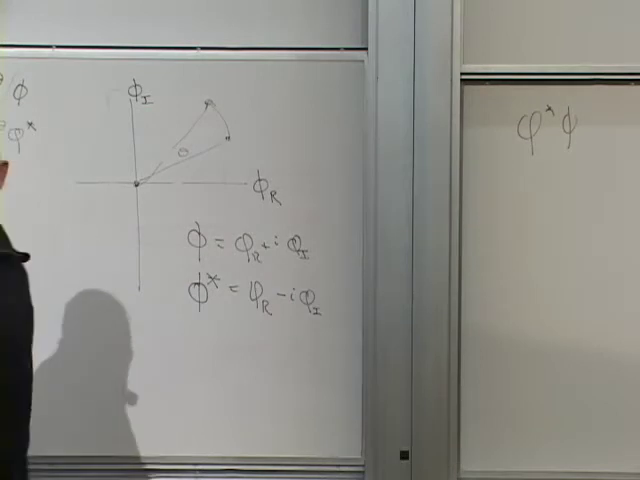
\includegraphics[width=0.80\textwidth]{lecture_07_figure_02.png}
\caption{Комплексное поле на внутренней плоскости \((\phi_R,\phi_I)\). На доске записаны разложения \(\phi\) и \(\phi^*\), а также инвариантный радиус \(\phi^*\phi\).}
\lectureframe{00:33:33}
\end{figure}

Воспользуемся лагранжианом
\begin{equation}
  \mathcal L
  =\partial_\mu\phi^*\,\partial^\mu\phi
   -V(\phi^*\phi).
  \label{eq:l07-complex-lagrangian}
\end{equation}
Для комплексного поля обычный множитель \(1/2\) отсутствует, поскольку этот единственный член уже содержит кинетические члены обеих вещественных компонент. Преобразование
\begin{equation}
  \phi'(x)=e^{i\theta}\phi(x),
  \qquad
  \phi^{*\prime}(x)=e^{-i\theta}\phi^*(x)
  \label{eq:l07-global-u1}
\end{equation}
поворачивает каждое значение поля на один и тот же угол. Здесь \(\theta\) постоянно в пространстве и времени. Штрих обозначает преобразованное поле; это не производная.

Поскольку \(\theta\) постоянно,
\begin{equation}
  \partial_\mu\phi'=e^{i\theta}\partial_\mu\phi,
  \qquad
  \partial_\mu\phi^{*\prime}
  =e^{-i\theta}\partial_\mu\phi^*.
\end{equation}
В кинетическом члене фазы сокращаются, и
\(\phi^{*\prime}\phi'=\phi^*\phi\). Следовательно, любой потенциал, зависящий только от
\(\phi^*\phi\), обладает той же симметрией. Член, зависящий только от \(\phi_R\),
выбирал бы направление во внутренней плоскости и явно нарушал бы симметрию.

\subsection{Точечный минимум и окружность минимумов}

Существуют два качественно различных симметричных потенциала. У первого
единственный минимум находится в начале координат, например
\begin{equation}
  V_{\rm unbroken}=m^2\phi^*\phi,
  \qquad m^2>0.
\end{equation}
Его график представляет собой параболоид с вращательной симметрией. Вакуум \(\phi=0\)
остаётся неизменным при любом повороте, так что симметрия не нарушена.

Теперь выберем
\begin{equation}
  V_{\rm broken}
  =-a\,\phi^*\phi+b(\phi^*\phi)^2,
  \qquad a,b>0.
  \label{eq:l07-mexican-hat}
\end{equation}
Отрицательный квадратичный член уводит поле от начала координат, тогда как
положительный квартичный член не позволяет ему уйти на бесконечность. Обозначив
\(r^2=\phi^*\phi\), из условия минимума получаем
\begin{equation}
  \frac{dV}{d(r^2)}=-a+2br^2=0,
  \qquad
  r^2=f^2=\frac{a}{2b}.
  \label{eq:l07-vacuum-radius}
\end{equation}
Следовательно, минимумы образуют окружность. Потенциал полностью инвариантен относительно
вращений, однако однородное основное состояние должно выбрать одну точку на
этой окружности.

\begin{figure}[htbp]
\centering
\includegraphics[width=0.72\textwidth]{lecture_07_figure_06.png}
\caption{Потенциал, нарушающий симметрию, изображён как поверхность вращения.
Начало координат неустойчиво, а вырожденные минимумы образуют кольцевой жёлоб.}
\lectureframe{00:37:25}
\end{figure}

Представьте поле как маленькую стрелку в этой внутренней плоскости в каждой точке
обычного пространства. Потенциал требует, чтобы каждая стрелка имела длину \(f\). Энергия
градиента требует, чтобы соседние стрелки были направлены почти одинаково.
Поэтому в основном состоянии угол всюду одинаков, но никакой угол не
выделен самим законом. Это и есть непрерывное спонтанное нарушение симметрии.

\section{От доменной стенки к плавному закручиванию}

Повторим граничный эксперимент. На левой границе зафиксируем поле в
вакуумной точке \(A\); на правой зафиксируем его в другой вакуумной точке \(B\). Локализованный
скачок сделал бы градиент большим. Однако, в отличие от дискретного случая,
поле может оставаться на дне потенциала, непрерывно изменяясь по
окружности.

При низкой энергии запишем поле как \(\phi=f e^{i\alpha(x)}\). В одном пространственном
измерении соответствующая энергия равна
\begin{equation}
  E[\alpha]
  =f^2\int_0^L dx\,\left(\frac{d\alpha}{dx}\right)^2.
  \label{eq:l07-angle-functional}
\end{equation}
При фиксированных углах на концах вариация даёт
\begin{equation}
  \frac{d^2\alpha}{dx^2}=0,
  \qquad
  \alpha(x)=\alpha_A+
    \frac{\alpha_B-\alpha_A}{L}\,x.
  \label{eq:l07-linear-twist}
\end{equation}
Предпочтительная конфигурация равномерно распределяет закручивание по всему образцу.
Её энергия масштабируется как
\begin{equation}
  E_{\rm twist}
  =f^2\frac{(\alpha_B-\alpha_A)^2}{L},
  \label{eq:l07-twist-energy}
\end{equation}
так что её можно сделать сколь угодно малой, увеличивая \(L\).

\begin{figure}[htbp]
\centering
\begin{adjustbox}{max width=\linewidth}
\begin{tikzpicture}[x=0.95cm,y=0.95cm]
  \begin{scope}
    \draw[->] (0,0) -- (6.2,0) node[right] {$x$};
    \draw[->] (0,0) -- (0,3.5) node[above] {$\alpha(x)$};
    \draw[very thick,blue!70!black] (0.45,0.65) -- (5.7,2.85);
    \fill (0.45,0.65) circle (1.8pt) node[left] {$\alpha_A$};
    \fill (5.7,2.85) circle (1.8pt) node[right] {$\alpha_B$};
    \node at (3.1,-0.65) {physical space};
  \end{scope}
  \begin{scope}[xshift=9.2cm,yshift=1.65cm]
    \draw[thick] (0,0) circle (1.8);
    \fill (1.55,-0.92) circle (1.8pt) node[below right] {$A$};
    \fill (-0.45,1.74) circle (1.8pt) node[above] {$B$};
    \draw[very thick,blue!70!black,-{Latex[length=2.5mm]}]
      (1.55,-0.92) arc[start angle=-31,end angle=104,radius=1.8];
    \node at (0,-2.35) {vacuum circle};
  \end{scope}
\end{tikzpicture}
\end{adjustbox}
\caption{Одна и та же низкоэнергетическая конфигурация в двух описаниях. Угол
линейно меняется в физическом пространстве, тогда как поле проходит по короткой дуге
вакуумной окружности во внутреннем пространстве.}
\end{figure}

\begin{classroomqa}
\audiencequestion{Вокруг окружности можно пройти двумя путями. По какому пути идёт
поле и может ли оно застрять на более длинном?
\lecturetimestamp{00:41:54}}
\lecturerresponse{Для общих положений концов более короткий угловой путь даёт
меньший градиент и, следовательно, меньшую энергию. Для диаметрально противоположных
концов две простейшие траектории вырождены. Конфигурация, подготовленная
медленным перемещением одного конца, может сохранить лишнюю намотку и оказаться
запертой за энергетическим барьером, но для заданной пары обычных граничных точек
основным состоянием является кратчайший путь без дополнительной намотки.}
\end{classroomqa}

\begin{classroomqa}
\audiencequestion{Может ли траектория уйти с дна жёлоба и срезать через внутреннюю
область, чтобы в целом стать короче?\lecturetimestamp{00:43:32}}
\lecturerresponse{В низкоэнергетическом режиме и для длинного образца невыгодно
подниматься по радиальному потенциалу. Удерживание радиуса на его вакуумном значении и
линейное изменение угла минимизируют эффективную энергию, как показывает
приведённое выше вычисление вариационным исчислением. Для конечной системы с
конкретным потенциалом можно минимизировать радиальное и угловое движение совместно, но
вывод Голдстоуна относится к пределу сколь угодно большой длины волны, в котором
выигрывает гладкое движение вдоль жёлоба.}
\end{classroomqa}

\begin{classroomqa}
\audiencequestion{Что изменится, если кольцевой жёлоб наклонить так, что одно
значение угла окажется ниже?\lecturetimestamp{00:44:33}}
\lecturerresponse{Тогда симметрия явно нарушена. Одна точка становится
истинным основным состоянием, движение вдоль окружности приобретает возвращающую силу,
и угловое возбуждение уже не является точно безмассовым.}
\end{classroomqa}

\section{Масса как цена колебания с нулевым импульсом}

Плавное закручивание выявляет поле, энергия которого обусловлена только градиентами. Чтобы
понять, почему это означает безмассовую частицу, сравним релятивистское
дисперсионное соотношение
\begin{equation}
  \omega^2=\bm{k}^2+m^2.
  \label{eq:l07-dispersion}
\end{equation}
Волна \(e^{i(\bm{k}\cdot\bm{x}-\omega t)}\) несёт импульс \(\bm{k}\).
Если \(m=0\), её энергия стремится к нулю, когда длина волны стремится к бесконечности:
\(\omega=|\bm{k}|\to0\). Если \(m\ne0\), то пространственно однородная мода
\(\bm{k}=0\) всё же осциллирует с частотой \(\omega=m\). Масса — это
неустранимая энергия при нулевом импульсе.

То же различие видно и в лагранжиане. Член
\begin{equation}
  -\frac12m^2\varphi^2
\end{equation}
создаёт возвращающую силу даже для однородного смещения. У поля, содержащего
только производные члены, такой возвращающей силы нет: увеличивайте его длину волны,
и его градиентная энергия стремится к нулю.

\subsection{Полярные переменные разделяют две моды}

Запишем комплексное поле в нарушенной фазе как
\begin{equation}
  \phi(x)=\rho(x)e^{i\alpha(x)}.
  \label{eq:l07-polar}
\end{equation}
И \(\rho\), и \(\alpha\) являются полями. Дифференцирование даёт
\begin{align}
  \partial_\mu\phi
  &=e^{i\alpha}
    \left(\partial_\mu\rho+i\rho\,\partial_\mu\alpha\right),\\
  \partial_\mu\phi^*
  &=e^{-i\alpha}
    \left(\partial_\mu\rho-i\rho\,\partial_\mu\alpha\right).
\end{align}
Перекрёстные члены сокращаются, и остаётся
\begin{equation}
  \partial_\mu\phi^*\,\partial^\mu\phi
  =(\partial_\mu\rho)(\partial^\mu\rho)
   +\rho^2(\partial_\mu\alpha)(\partial^\mu\alpha).
  \label{eq:l07-polar-kinetic}
\end{equation}
Поскольку \(\phi^*\phi=\rho^2\),
\begin{equation}
  \mathcal L
  =(\partial\rho)^2+\rho^2(\partial\alpha)^2-V(\rho^2).
  \label{eq:l07-polar-lagrangian}
\end{equation}
Потенциал содержит \(\rho\), но не \(\alpha\). Это отсутствие и есть
симметрия в её наиболее полезной форме.

\begin{figure}[htbp]
\centering
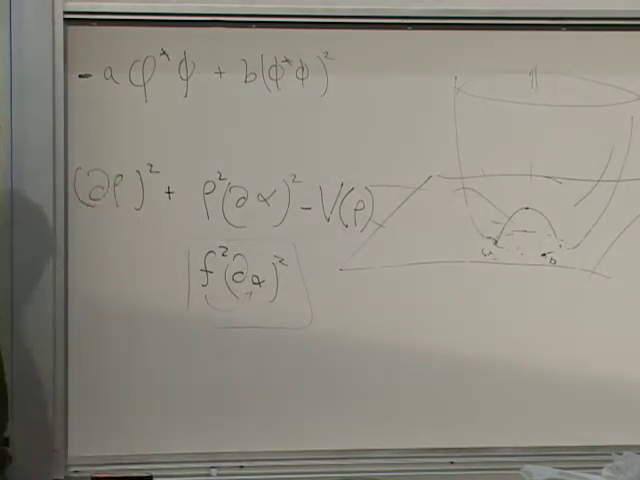
\includegraphics[width=0.88\textwidth]{lecture_07_figure_03.png}
\caption{Лагранжиан поля в полярных переменных, выделенный рамкой низкоэнергетический угловой член и
потенциал, нарушающий симметрию. Радиальное движение поднимается по потенциалу; угловое
движение идёт вдоль жёлоба.}
\lectureframe{00:56:40}
\end{figure}

Для возбуждения с очень малой энергией поле остаётся близким к
\(\rho=f\). Тогда
\begin{equation}
  \mathcal L_{\rm angular}
  \simeq f^2(\partial_\mu\alpha)(\partial^\mu\alpha).
\end{equation}
Определим канонически нормированное угловое поле, с точностью до соглашения о множителях \(1/2\), как
\begin{equation}
  \beta=\sqrt{2}\,f\alpha,
  \qquad
  \mathcal L_{\rm angular}
  =\frac12(\partial_\mu\beta)(\partial^\mu\beta).
  \label{eq:l07-goldstone-field}
\end{equation}
Члена \(\beta^2\) нет. Кванты этого углового поля безмассовы.
Это бозоны Голдстоуна.

Радиальное поле ведёт себя иначе. Если сразу всюду сместить \(\rho\) от \(f\),
оно скатится обратно, пройдёт через минимум и будет осциллировать около жёлоба. Если
\(\rho=f+h\), то разложение формулы ~\eqref{eq:l07-mexican-hat} даёт
\begin{equation}
  V(f+h)=V(f)+\frac12m_h^2h^2+\cdots,
\end{equation}
так что \(h\) имеет массу. Геометрически угловое направление плоское, а
радиальное — искривлённое.

\begin{classroomqa}
\audiencequestion{Если поле смещено радиально, просто ли оно падает
обратно вниз и что происходит потом?\lecturetimestamp{00:57:10}}
\lecturerresponse{Если углового движения нет, оно падает к минимуму,
проходит через него и осциллирует радиально. Однородное колебание имеет нулевой
пространственный импульс, но ненулевую частоту; эта частота и есть масса
радиального возбуждения. Однородное угловое смещение, напротив, приводит к
другому вакууму и не имеет возвращающей силы.}
\end{classroomqa}

В рассматриваемом примере содержание принципа Голдстоуна таково:
спонтанное нарушение непрерывной глобальной симметрии порождает безмассовую моду
для каждого независимого плоского направления многообразия вакуума.
\editorialnote{Это утверждение предполагает обычные условия релятивистской
теории поля. В нерелятивистских многочастичных системах подсчёт и
дисперсия мод Намбу--Голдстоуна могут быть более тонкими, но вывод лекции о
длинноволновом пределе остаётся верным для этой релятивистской модели \(U(1)\).}

\section{Спиновые волны, струны и звук}

Теорема абстрактна, но её механизм хорошо знаком. В изотропном
ферромагните все спины можно повернуть совместно, не изменяя энергии.
Если позволить ориентации очень медленно меняться по образцу, получится
спиновая волна. Её энергетическая цена обращается в нуль вместе с её волновым
числом, так что это мода Голдстоуна нарушенной симметрии вращения спинов.

Длинная упругая струна даёт другую наглядную картину. Пренебрежём гравитацией и закрепим
концы так, чтобы всю струну можно было сдвигать по вертикали. Однородный
вертикальный сдвиг не требует энергии. Если позволить ему медленно меняться вдоль
струны, он превращается в длинноволновую поперечную волну. Однородная
операция симметрии превращена в плавную деформацию, зависящую от
положения.

\begin{figure}[htbp]
\centering
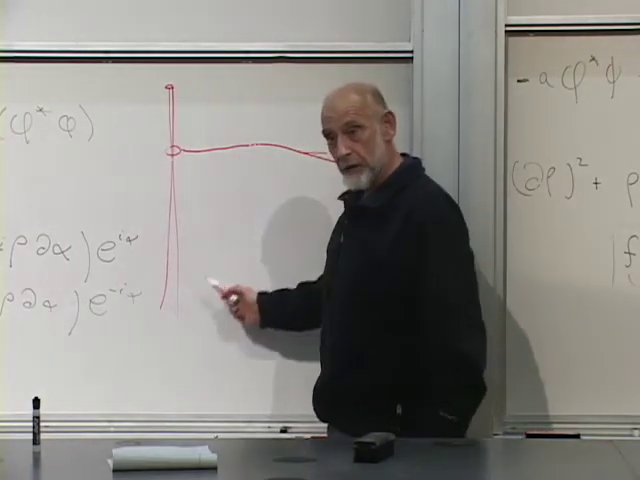
\includegraphics[width=0.68\textwidth]{lecture_07_figure_04.png}
\caption{Медленно меняющийся профиль струны, нарисованный при аналогии с модой Голдстоуна.
Физически важен малый наклон длинноволновой деформации, а не вертикальное положение
кривой.}
\lectureframe{01:04:19}
\end{figure}

\begin{classroomqa}
\audiencequestion{Может ли струна нести энергию колебаний, имея при этом нулевой
импульс?\lecturetimestamp{01:04:41}}
\lecturerresponse{Нужно различать вертикальный механический импульс и
волновой импульс вдоль струны. Стоячая волна может иметь нулевой суммарный импульс,
поскольку она является суперпозицией мод с \(+k\) и \(-k\), и при этом всё же
нести энергию. В аналогии с теорией поля импульс относится к волновому
числу вдоль оси; вертикальное смещение представляет внутреннюю координату
поля.}
\end{classroomqa}

Пружинка-слинки дает продольный аналог. Сдвиньте всю идеализированную бесконечную пружинку вдоль ее оси — и ничего не изменится. Сдвиньте соседние части на немного разные величины — и получится слабая волна сжатия. В твердом теле или жидкости длинноволновой звук аналогично возникает из коллективных смещений и изменений плотности. Спиновые волны, поперечные волны на струне и звук — не одно и то же микроскопическое возбуждение, но у них есть решающая общая черта: однородное непрерывное преобразование не требует энергии, а его медленно меняющийся вариант становится мягкой модой.
\editorialnote{В кристалле акустические фононы обычно описывают как моды Намбу--Голдстоуна, возникающие при спонтанном нарушении непрерывных трансляций. Струна и пружинка-слинки — механические аналогии, используемые в лекции, чтобы выявить ту же структуру энергии, зависящую только от производных.}

Терминология здесь достаточно важна, чтобы позволить себе короткую шутку в аудитории: это \emph{Голдстоуна}-бозоны, названные в честь Джеффри Голдстоуна, а не калибровочные бозоны. В лекции отмечается, что Голдстоун был другом Сасскинда, после чего изложение переходит к действительно другой теме — калибровочной инвариантности.

\section{От глобальной фазовой симметрии к калибровочной симметрии}

Симметрия фаз \(U(1)\) уже появлялась в курсе как симметрия, связанная с сохранением заряда. Поля заряженных частиц комплексны, и умножение такого поля на общую фазу оставляет глобальную теорию неизменной. Для наглядности можно говорить об электрическом заряде, хотя он может представлять и другое квантовое число \(U(1)\). Настоящий фотон безмассов; конечная цель — фотоноподобное поле, такое как массивное \(Z\).

Новый вопрос состоит в том, может ли
\begin{equation}
  \phi'(x)=e^{i\theta(x)}\phi(x)
  \label{eq:l07-local-u1}
\end{equation}
быть симметрией, когда \(\theta\) произвольно меняется в пространстве-времени. Функция \(\theta(x)\) — это параметр преобразования, а не дополнительное динамическое поле. Проверим это предложение, продифференцировав:
\begin{equation}
  \partial_\mu\phi'
  =e^{i\theta}
   \left[\partial_\mu\phi+i(\partial_\mu\theta)\phi\right].
  \label{eq:l07-local-derivative}
\end{equation}
Этот дополнительный член отсутствовал при постоянной \(\theta\). Для комплексно-сопряженного поля
\begin{equation}
  \partial_\mu\phi^{*\prime}
  =e^{-i\theta}
   \left[\partial_\mu\phi^*-i(\partial_\mu\theta)\phi^*\right].
\end{equation}
Их произведение равно
\begin{align}
  \partial_\mu\phi^{*\prime}\partial^\mu\phi'
  ={}&
  \partial_\mu\phi^*\partial^\mu\phi
  i\left(
      \phi\,\partial_\mu\phi^*
      -\phi^*\partial_\mu\phi
    \right)\partial^\mu\theta
  \nonumber\\
  &+\phi^*\phi\,
    \partial_\mu\theta\,\partial^\mu\theta.
  \label{eq:l07-local-failure}
\end{align}
Потенциал остается инвариантным, потому что инвариантно \(\phi^*\phi\), но обычный кинетический член перестает быть инвариантным. Глобальная симметрия не стала автоматически локальной.

\begin{classroomqa}
\audiencequestion{На картинке с «мексиканской шляпой» означает ли эта неудача, что вдоль кругового желоба есть бугорки?\lecturetimestamp{01:19:37}}
\lecturerresponse{Нет. Потенциал может оставаться совершенно плоским в угловом направлении. Дополнительная энергетическая цена возникает из-за градиентов, когда фаза различается от одной точки пространства-времени к другой. Это не гофрировка желоба; это обычный член с производной, который обнаруживает пространственную неоднородность.}
\end{classroomqa}

\subsection{Компенсирующее векторное поле}

В природе взаимодействия фотона, \(W\), \(Z\) и глюонов организованы локальными калибровочными симметриями, а не просто жесткими преобразованиями. Чтобы локальная фазовая операция стала симметрией, нужно расширить теорию, введя четырехвекторное поле \(A_\mu\). В электромагнетизме \(A_0\) — скалярный потенциал, а три пространственные компоненты образуют векторный потенциал. Из их производных строятся электрическое и магнитное поля.

Выберите внутренне согласованное соглашение
\begin{equation}
  \phi'=e^{i\theta}\phi,
  \qquad
  A'_\mu=A_\mu-\partial_\mu\theta,
  \qquad
  D_\mu=\partial_\mu+iA_\mu.
  \label{eq:l07-gauge-convention}
\end{equation}
На доске при проверке компенсации меняется знак; уравнение
\eqref{eq:l07-gauge-convention} одновременно фиксирует все три знака. Константа калибровочного
взаимодействия и заряд временно поглощены в \(A_\mu\).
\editorialnote{При явном указании заряда \(q\) и константы связи \(g\) можно записать
\(D_\mu=\partial_\mu+igqA_\mu\) и
\(A'_\mu=A_\mu-(gq)^{-1}\partial_\mu\theta\). На лекции эти
константы опущены, чтобы компенсация оставалась наглядной.}

Для сопряжённого поля
\begin{equation}
  D_\mu\phi^*=\partial_\mu\phi^*-iA_\mu\phi^*.
\end{equation}
Теперь
\begin{align}
  D'_\mu\phi'
  &=
  \left(\partial_\mu+iA'_\mu\right)e^{i\theta}\phi
  \nonumber\\
  &=
  e^{i\theta}
  \left[
    \partial_\mu\phi+i(\partial_\mu\theta)\phi
    +i(A_\mu-\partial_\mu\theta)\phi
  \right]
  \nonumber\\
  &=e^{i\theta}D_\mu\phi.
  \label{eq:l07-covariant-transform}
\end{align}
Нежелательная производная от \(\theta\) компенсируется преобразованием
\(A_\mu\). Аналогично,
\begin{equation}
  D'_\mu\phi^{*\prime}=e^{-i\theta}D_\mu\phi^*.
\end{equation}
Их произведение инвариантно. Прилагательное \emph{ковариантная} означает, что
производная преобразуется тем же простым образом, что и само поле.

\section{Динамика калибровочного поля}

Введение \(A_\mu\) лишь для исправления производной оставило бы его без
собственной динамики. Калибровочно-инвариантная напряжённость поля равна
\begin{equation}
  F_{\mu\nu}
  =\partial_\mu A_\nu-\partial_\nu A_\mu.
  \label{eq:l07-field-strength}
\end{equation}
Она антисимметрична, поэтому \(F_{\mu\mu}=0\).

Её время--пространственные компоненты содержат
электрическое поле, тогда как пространство--пространственные компоненты содержат магнитное
поле. В привычных обозначениях с трёхмерными векторами плотность энергии
электромагнитного поля пропорциональна \(\bm E^2+\bm B^2\), тогда как лоренцев лагранжиан
пропорционален \(\bm E^2-\bm B^2\); знаки зависят от принятого соглашения
о метрике.

\begin{classroomqa}
\audiencequestion{Каковы энергия и лагранжиан электромагнитного
поля?\lecturetimestamp{01:33:20}}
\lecturerresponse{Энергия строится из \(E^2+B^2\); в лагранжиане используется
\(E^2-B^2\). В ковариантной форме последняя величина записывается как
\(F_{\mu\nu}F^{\mu\nu}\), умноженное на стандартный коэффициент. Антисимметричный тензор — это четырёхмерный
ротор векторного потенциала.}
\end{classroomqa}

Напряжённость поля сама по себе калибровочно-инвариантна:
\begin{align}
  F'_{\mu\nu}
  &=
  \partial_\mu(A_\nu-\partial_\nu\theta)
  -\partial_\nu(A_\mu-\partial_\mu\theta)
  \nonumber\\
  &=
  F_{\mu\nu}
  -\partial_\mu\partial_\nu\theta
  +\partial_\nu\partial_\mu\theta
  =F_{\mu\nu}.
  \label{eq:l07-field-strength-invariant}
\end{align}
Последнее равенство следует из того, что обычные смешанные частные производные
коммутируют. Поэтому стандартный калибровочно-инвариантный лагранжиан имеет вид
\begin{equation}
  \boxed{
  \mathcal L
  =(D_\mu\phi)^*D^\mu\phi
  -V(\phi^*\phi)
  -\frac14F_{\mu\nu}F^{\mu\nu}}
  \label{eq:l07-scalar-qed}
\end{equation}
с точностью до соглашений о знаках и нормировке, выбранных для метрики.

\begin{figure}[htbp]
\centering
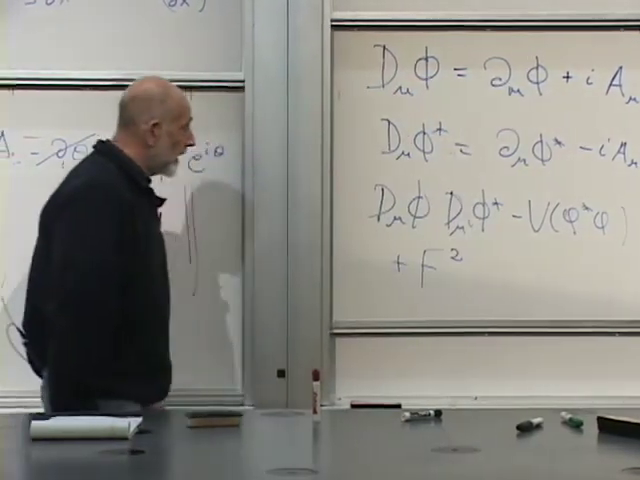
\includegraphics[width=0.84\textwidth]{lecture_07_figure_05.png}
\caption{Ковариантные производные и построенный на доске калибровочно-инвариантный
лагранжиан. Численные множители там опущены, чтобы структура
преобразований оставалась наглядной.}
\lectureframe{01:38:45}
\end{figure}

Эта конструкция повышает глобальную симметрию \(U(1)\) до локальной, но делает это ценой --- или, физически говоря, даруя нам --- новое векторное поле.
В абелевом примере этим полем является электромагнитный потенциал.

\begin{classroomqa}
\audiencequestion{Лагранжиан, с которого мы начали, использовал обычные производные. Почему
мы вправе заменить их ковариантными производными и назвать результат
настоящей теорией?\lecturetimestamp{01:42:55}}
\lecturerresponse{Мы строим другую, расширенную теорию: заряженная
материя плюс калибровочное поле. Локальная калибровочная инвариантность определяет их взаимодействие.
Получающаяся квантовая теория представляет собой согласованную математическую структуру и согласуется
с тем, как природа организует фотон и слабые калибровочные поля. Простое несогласованное введение
взаимодействия релятивистского векторного поля может привести к нефизическим
поляризациям и нарушениям вероятностной интерпретации, так что калибровочный принцип не является
косметической перезаписью старой теории свободного скалярного поля.}
\end{classroomqa}

\begin{classroomqa}
\audiencequestion{То есть добавление нового поля и есть главное обоснование этой модификации?\lecturetimestamp{01:44:57}}
\lecturerresponse{Да. Без \(A_\mu\) производная локально повернутого поля содержит нескомпенсированный \(\partial_\mu\theta\). При наличии \(A_\mu\) и закона его преобразования сокращение происходит. На геометрическом языке \(A_\mu\) — это связность на расслоении; эта более глубокая математика вполне реальна и полезна, но приведенная выше алгебра содержит ту часть, которая здесь нужна.}
\end{classroomqa}

\section{Почему запрещена затравочная масса калибровочного бозона}

Для обычного бозонного поля масса представляется квадратичным членом.
Естественно попытаться добавить
\begin{equation}
  \Delta\mathcal L_{\rm Proca}
  =\frac12m^2A_\mu A^\mu.
  \label{eq:l07-proca}
\end{equation}
Однако при \(A_\mu\mapsto A_\mu-\partial_\mu\theta\)
\begin{equation}
  A'_\mu A^{\mu\prime}
  =
  A_\mu A^\mu
  -2A^\mu\partial_\mu\theta
  +\partial_\mu\theta\,\partial^\mu\theta,
\end{equation}
поэтому формула~\eqref{eq:l07-proca} не является калибровочно-инвариантной. Мы не можем ввести массу в эту калибровочную теорию вручную, сохранив ее локальную симметрию.

\begin{figure}[htbp]
\centering
\includegraphics[width=0.72\textwidth]{lecture_07_figure_07.png}
\caption{Предлагаемый затравочный массовый член для векторного поля
\(\tfrac12m^2A_\mu A^\mu\). Именно то, что он неинвариантен при
\(A_\mu\mapsto A_\mu-\partial_\mu\theta\), и создает препятствие, ведущее к
механизму Хиггса.}
\lectureframe{01:39:48}
\end{figure}

В этом и состоит кажущийся тупик. Калибровочная инвариантность объясняет, почему фотон безмассов, и защищает теорию от нефизических степеней свободы, но \(W\) и
\(Z\) массивны. Выходом не может быть явная масса векторного поля. Она должна
возникать из полей, уже присутствующих в калибровочно-инвариантном лагранжиане.

\begin{classroomqa}
\audiencequestion{Само введение калибровочной инвариантности порождает
бозон Голдстоуна?\lecturetimestamp{01:45:51}}
\lecturerresponse{Нет. Бозон Голдстоуна возник, когда непрерывная
\emph{глобальная} симметрия была спонтанно нарушена, еще до введения векторного потенциала.
Как только симметрия становится локальной, изменяющуюся фазу можно
скомпенсировать с помощью \(A_\mu\). В калибровочной теории с нарушенной симметрией угловая мода больше
не является независимой безмассовой частицей; она обеспечивает дополнительную
поляризацию теперь уже массивного векторного поля. На следующей лекции это утверждение будет выведено,
а не просто объявлено.}
\end{classroomqa}

\begin{classroomqa}
\audiencequestion{Объясняет ли что-то из этого, почему реки меандрируют?
\lecturetimestamp{01:47:03}}
\lecturerresponse{О прямой связи здесь ничего не известно. Вихри в жидкости и даже
формы организмов, разумеется, можно описывать методами симметрии,
и не стоит удивляться, если идеи теории поля обнаруживаются в неожиданных
местах, но лекция не утверждает существования калибровочной теории речных меандров.}
\end{classroomqa}

\section{На этом лекция заканчивается}

Теперь у нас есть две составляющие, обещанные в начале. Непрерывная
глобальная симметрия, у которой вакуумы образуют окружность, имеет плоское угловое направление, и медленное
изменение вдоль него представляет собой безмассовое поле Голдстоуна. Локальная симметрия требует калибровочной
связности и ковариантных производных и запрещает прямую массу векторного
поля в формуле~\eqref{eq:l07-proca}.

Следующий шаг — использовать потенциал с нарушенной симметрией из уравнения~\eqref{eq:l07-mexican-hat} в калибровочно-инвариантной теории из уравнения~\eqref{eq:l07-scalar-qed}. Тогда одновременно происходят две вещи: отдельная частица Голдстоуна исчезает из физического спектра, а векторное поле приобретает массу. В обычном учебном изложении говорят, что калибровочная симметрия спонтанно нарушается; точнее, калибровочная избыточность сохраняется, а теория входит в фазу Хиггса с массивным векторным возбуждением.
\editorialnote{Локальная калибровочная симметрия — это избыточность описания, а не обычная физическая симметрия, действующая между различными наблюдаемыми состояниями. В лекции используется стандартное сокращённое выражение о спонтанном нарушении калибровочной симметрии. Калибровочно-инвариантное физическое утверждение — это перестройка степеней свободы в фазе Хиггса.}

Это и есть явление Хиггса. Мы его ещё не осуществили. В этой лекции была проделана необходимая, более трудная работа: задача сформулирована достаточно точно, так что её решение, когда оно появится, окажется неизбежным.
